\documentclass[11pt,a4paper]{article}
\usepackage[utf8]{inputenc}
\usepackage[german]{babel}
\usepackage[T1]{fontenc}
\usepackage{amsmath}
\usepackage{amsfonts}
\usepackage{amssymb}
\usepackage{graphicx}
\usepackage{color}
\usepackage[left=2cm,right=2cm,top=2cm,bottom=2cm]{geometry}
\author{Christian Weiß}
\title{Implementierung und Evaluirung eines SNMP Scanners}
\begin{document}
% -----------------------------------------------------------------------------------------------------------------------------------------
% Titelblatt
% -----------------------------------------------------------------------------------------------------------------------------------------
\begin{figure}	% Logo
	\centering
	
\includegraphics[scale=.7]{Bilder/hsa.jpg}
	\label{img:logo}
\end{figure}
	
\vspace{\fill}

\begin{center}
	
	\begin{Huge}
		Abschlussarbeit\linebreak
	\end{Huge}
	
	\vspace{\fill}
	
	\begin{Large}
		Fakultät für Informatik\linebreak
	\end{Large}
	
	\vspace{\fill}
	
	\begin{LARGE}
		Titel\linebreak
	\end{LARGE}
	
	\vspace{1cm}
	
	\begin{Huge}
		\textbf{Implementierung und Evaluation eines SNMP Scanners}\linebreak
	\end{Huge}
	
	\vspace{\fill}
	
	\begin{Large}
		\begin{tabular}{r l}
			Autor: & Christian Weiß \\
			Prüfer: & Prof. Dr. Winter \\
			Datum: & \today \\
		\end{tabular}
	\end{Large}
	
\end{center}	% END - Titleseite
\pagebreak

% -----------------------------------------------------------------------------------------------------------------------------------------
% Inhaltsverzeichnis
% -----------------------------------------------------------------------------------------------------------------------------------------
\tableofcontents

% -----------------------------------------------------------------------------------------------------------------------------------------
% Einleitung (Motivation)
% -----------------------------------------------------------------------------------------------------------------------------------------
%\setcounter{page}{1}
\section*{Einleitung}
Das Internet ist ein weltweiter Verbund von Rechnernetzwerken. Physikalisch besteht das Internet im Kernbereich aus einzelnen Netzwerken von Providern, Firmen und Universitäts- und Forschungsnetzwerke. Router verbinden diese Netzwerke miteinander.\\
Das Internet im Ganzen ist unbekannt. Selbst Netzbetreiber kennen nur einen kleinen Teil. Eine Verwaltung findet nur in den Subnetzen statt. Das macht eine Erfassung und Überwachung schwierig. Um den Zustand des Internet zu messen, sind viele Messstellen notwendig. Gut geeignet als Messstellen sind Endgeräte die sich regelmäßig Pakete durchs Internet schicken. Dieser Datenverkehr aus den Messungen kann Aufschluss über das Internet geben. Dafür wurde in der Hochschule eine App namens „Glimpse“ entwickelt, die auf allen erdenklichen Endgeräten installiert werden kann.
Glimpse verfügt über verschiedene Messmethoden, wie z.B. ein Bandbreitentest. Die Endgeräte sollen aus den Subnetzen, in denen sie sich befinden, die Bandbreite des Netzwerks zum Internet messen. Doch das Ergebnis einer solchen Messung kann keinen direkten Aufschluss zur Bandbreite geben. Waren zum Zeitpunkt der Messung noch andere Verbindungen aktive, so kann der gemessene Wert von der Bandbreite des Netzwerks stark Abweichen. Um nun eine bessere Einschätzung machen zu können, müsste man wissen, wie viele Verbindungen während der Messung bestanden haben. Diese Information hält ein Router in seinen Statistiken.\\
Es gibt verschiedene Protokolle mit denen Administratoren ihre Geräte im Netzwerk verwalten können. Darunter fallen Netconf und SNMP (Simple Network Management Protocol). Das Simple Network Management Protocol ist bereits weit verbreitet. Auf vielen Geräten wie Routern, Switches und Druckern ist vom Hersteller die Software bereits installiert. Ausgeliefert werden sie mit Standardpasswörtern, die von den Administratoren oft nicht geändert werden. Das bietet mir die Möglichkeit diese Geräte zu finden und auszulesen.
Findet sich im Subnetz von einem Glimpse-Client ein Gateway-Router, der mit den Standardpasswörtern läuft, können die Statistiken ausgelesen werden.
\pagebreak

% -----------------------------------------------------------------------------------------------------------------------------------------
% Geschichte
% -----------------------------------------------------------------------------------------------------------------------------------------
\section*{Geschichte}
„Die Geschichte des SNMP hängt stark mit der Geschichte des Internets zusammen.[…]
So entstand im Jahre 1987 das SGMP (Simple Gateway Monitoring Protocol), da zu damaliger Zeit das Verbinden der Gateways das Hauptproblem war. Gleichzeitig entstand noch ein anderes Protokoll mit dem Namen HEMS (High Level Management Entity System), dessen Entwicklung schon länger zurückreichte. Allerdings fand dieses keine breite Unterstützung im Gegensatz zu dem SGMP, das schon zu dieser Zeit anfing, sich durchzusetzen. Ein weiterer Ansatz lag in einem OSI basierten Protokoll CMIP (Common Management Information Protocol) das auf TCP Protokoll aufgesetzt werden sollte und somit den Namen CMOT erhielt (CMIP over TCP). Aufgrund der geringen Durchsetzung von HEMS wurden nur SGMP und CMOT weiterentwickelt, ersteres, weil es schon weit verbreitet war und zweiteres, weil es auf einem langen ISO-standardisierten Untergrund aufbaute. Später sollten beide zu einem Protokoll verschmelzen.
1988 brachten die Entwickler um SGMP das RFC 1065 Structure of Managment Information [MR88b], RFC 1066 Managment Information Base [MR88a] und RFC 1067 Simple Network Managment Protocol [CFSD88] heraus, was dann 1989 zu recommended erklärt wurde, welches einem quasi-Standard entspricht und ab hier auch schon den Namen SNMP trägt. […]
SNMPv2 war allerdings von seinem Sicherheitsstandard her zu komplex, so dass dies keine breite Zustimmung fand und so wurde 1996 SNMPv2 nur mit dem Sicherheitsmanagement aus SNMPv1 noch mal als RFC eingereicht, was dann SNMPv2c genannt wurde. Doch auch diese Lösung wurde nicht als zufriedenstellend empfunden und so entstanden die beiden Standards SNMPv2u und SNMPv2*, die das Sicherheitsproblem lösen sollten.
Als letztes ist noch SNMPv3, RFC 2272-2275, zu erwähnen, das als Nachfolger von SNMPv2 zu verstehen ist, aber zusätzlich noch die Vereinigung von SNMPv2u und SNMPv2* bewirken soll [Bla97]. Diese wurde 1998 zum Proposed Internet Standard und dann 1999 zum Draft Internet Standard.“
\cite{history}
\pagebreak

% -----------------------------------------------------------------------------------------------------------------------------------------
% Netzwer Management
% -----------------------------------------------------------------------------------------------------------------------------------------
\section*{Netzwerk Management}
„Netzwerkmanagement beinhaltet die Installation, Integration und Koordination von Hardware, Software und menschlichen Elemente zum Überwachen, Testen, Abfragen, Konfigurieren, Analysieren, Bewerten und Kontrollieren des Netzwerks und seiner Element-Ressourcen, um die Anforderungen in Bezug auf Performance im Betrieb und Dienstqualität zu angemessenen Kosten zu erfüllen.“
\cite{netmanagement}
\linebreak
Netzwerkmanagement bedeutet, alle managebaren Entitäten zu Verwalten und Überwachen. Bei den Entitäten handelt es sich im wesentlichen um Router, Switches, Drucker und Server. Um diese Geräte veralten zu können muss sich ein Management System Informationen über den Status dieser Geräte im Netzwerk beschaffen können. Damit lassen sich die Information, die übers Netzwerk ausgetauscht werden, in zwei Kategorien einteilen. Es werden Nachrichten versandt, die über den Status einer Resource informieren und das Management System muss Kommandos an die Ressourcen senden können. Die Nachrichten über den Status können vom Management System angefordert sein, können aber auch vom Gerät selbst als Warnung bei einer Fehlfunktion verschickt werden. Das Management System kann mit Kommandos an Entitäten reagieren um einer Fehlfunktion entgegen zu wirken.
Die folgende Abbildung zeigt eine allgemeine Darstellung einer Netzwerkmanagementarchitektur mit ihren Hauptkomponenten. Die verwaltende Einheit als Rechner oder Notebook (NMS) und verwaltete Geräte mit ihren Agenten (A).
\linebreak
\begin{figure}[h]
	\centering
	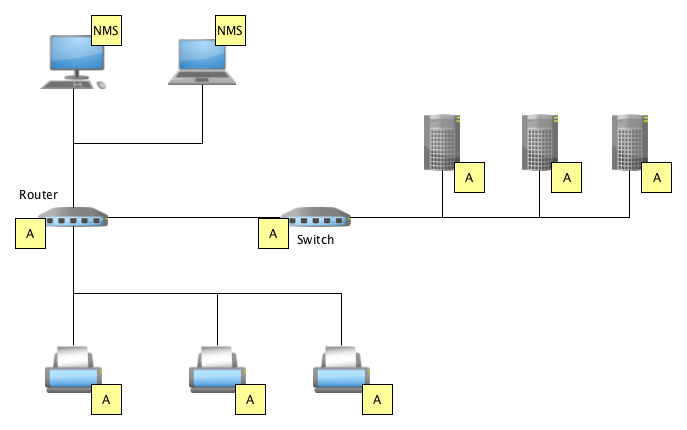
\includegraphics[scale=.5]{Bilder/Netzwerk.png}
	\caption{Beispiel Netzwerk mit allen Entitäten.}
\end{figure}
\linebreak

% -----------------------------------------------------------------------------------------------------------------------------------------
% Netzwerk Management System
% -----------------------------------------------------------------------------------------------------------------------------------------
\section*{Network Management Station}
Eine NMS ist ein Rechner der im selben Netzwerk angesiedelt ist wie die Agenten mit denen es kommuniziert. Auf diesem Rechner läuft eine Software, die dem Administrator das Überwachen und Konfigurieren seiner Geräte im Netzwerk erlaubt. Eine NMS kann auch automatisiert sein und auf Fehlermeldungen der Agenten reagieren.
\linebreak

% -----------------------------------------------------------------------------------------------------------------------------------------
% Agent
% -----------------------------------------------------------------------------------------------------------------------------------------
\section*{Agenten}
Ein Agent ist ein Softwaremodul, dass auf einem netzwerkfähigem Gerät installiert ist. Diese Software bildet die Schnittstelle zwischen dem Gerät und dem Managementsystem. Ein NMS kann einen Request an den Agenten senden um den Status einer Resource zu erfragen. Der Agent liest die angeforderten Informationen aus seinem Wirt aus. Diese Informationen packt der Agent in einen RequestResponse und antwortet damit dem NMS. Die Eigenschaften eines Gerätes, welches von einem Agenten verwaltet wird, können vom NMS auch verändert werden. Zu den Informationen, die der Agent überwacht und übermitteln kann, gehören Konfigurationsdaten, Statusinformationen und Statistikwerte.
Kritische Eigenschaften eines Gerätes können vom Agent permanent überwacht werden. Triftet ein Wert einer Überwachten Eigenschaft in einen kritischen Bereich ab, kann das der Agent registrieren. Er reagiert sofort und sendet eine Warnung an das NMS.
Jeder Agent hat dazu eine Management Information Base (MIB) in der die Werte spezifiziert sind, die er verwalten und überwachen kann. Die Einträge in der MIB verweisen auf die Managed Objects vom Gerät.
\linebreak
\begin{figure}[h]
	\centering
	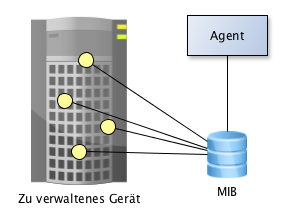
\includegraphics[scale=.7]{Bilder/Agent.png}
	\caption{EIn Agent und seine Managed Objects aus der MIB}
\end{figure}
\linebreak

% -----------------------------------------------------------------------------------------------------------------------------------------
% Agent
% -----------------------------------------------------------------------------------------------------------------------------------------
\section*{Management Information Base (MIB)}
Die Management Information Base (MIB) enthält alle Managed Objects, die ein Agent später referenzierten kann. Die einzelnen Objekte müssen in der MIB detailliert beschrieben werden. Jedes Object erhält seine eigenen Zugriffsrechte, die später für die Anfragen von einem NMS an den Agenten gelten sollen. Damit durch ein NMS gezielt solche Objekte angesprochen werden können, erhalten die Managed Objects eine eindeutige Object ID (OID). Zudem sind zu bestimmen mit welchem Datentype der Status des Objekts anzugeben ist und es es gibt eine Beschreibung für das Objekt in Textform.
Die Module und Objekte einer MIB sind angeordnet in Baumform und können mit der OID referenziert werden. Ein Identifier zu einem Managed Object im Baum besteht aus Nummern und kann z.B. so aussehen: „.1.3.6.1.2.1.1“. Die Länge der OID bestimmt die Tiefe im Baum. Eine einzelne Nummer gibt Auskunft über das Blatt auf horizontaler Ebene. Die Blätter tragen auch Namen. So kann eine OID auch wie folgt beschrieben werden: „.iso.org.dod.mgmt.mib-2.system.sysDescr.0“.
Die Managed Objects einer MIB werden in der Syntax, die von der SMI vorgegeben wird, in einer ASCII-Datei abgelegt. Diese Datei kann von einem MIB-Compiler für die Verwendung durch einen Agenten aufbereitet werden.
\linebreak
\begin{figure}[h]
	\centering
	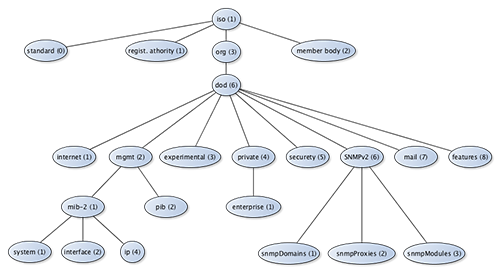
\includegraphics[scale=1]{Bilder/MIB.png}
	\caption{Die grobe Struktur des MIB-Baumes}
\end{figure}

% -----------------------------------------------------------------------------------------------------------------------------------------
% Structure of Management Information SMI
% -----------------------------------------------------------------------------------------------------------------------------------------
\section*{Structure of Management Information (SMI)}
Die SMI ist eine Sprache zur Beschreibung der MIB’s und wurde für SNMP entwickelt. Damit lassen sich die Module, Managed Objects und Notifications für die MIB erstellen. Die SMI legt dazu die Syntax fest, mit der eine MIB beschrieben werden kann. Außerdem sind verschiedene Datentypen wie INTEGER, Gauge, Counter64 und viele mehr definiert. Ansonsten ist die SMI ein Auszug aus der ASN.1.
Ein Beispiel für einen MIB-Eintrag in der Form, wie sie von der SMI vorgegeben wird:
\linebreak
\color{red}
neuesObj OBJECT-TYPE\\
		SYNTAX Ein Datentype aus der ASN.1 oder Abgeleitet.\\
		ACCESS read-only\\
		STATUS mandatory\\
		DESCRIPTION\\
			„Eine detaillierte Beschreibung dieses Objects“\\
		::= { internet 7 }\\
\color{black}
Damit würde ein Eintrag im Baum entstehen, der  wie folgt zu erreichen ist: iso.org.dod.internet.neuesObj\\
und als Object Identifier : 1.3.6.1.7.0

% -----------------------------------------------------------------------------------------------------------------------------------------
% Abstract Syntax Notation One ASN.1
% -----------------------------------------------------------------------------------------------------------------------------------------
\section*{Abstract Syntax Notation One (ASN.1)}
Zwischen den verschiedenen Geräten im Netzwerk kann es zu Inkompatibilitäten kommen. Die Hardware oder auch die installierte Software kann für die Daten unterschiedliche Darstellungen verwenden. Ein Beispiel dafür ware Big Endian und Little Endian. Bei der Kommunikation mit SNMP zwischen den Agenten und dem NMS müssen die Daten jedoch klar definiert sein. SNMP setzt für die Kompatibilität auf eine Teilmenge der ASN.1.
Die ASN.1 bietet einen Standard zur Definition von Datentypen und deren Werte. Ein Datentype ist eine Art von Information. Eine Information kann Beispielsweise eine Zahl, ein Text, ein Bilder oder auch ein Video sein. Für diese Informationen sollen Datentypen bereitgestellt werden. Ein hingegen Wert ist eine Instanz von einem dieser Datentypen. In der ASN.1 sind verschiede primitive Datentypen und deren Werte beschrieben. Außerdem finden sich Regeln um einfache Datentypen zu kombinieren, wodurch man komplexere Typen erzeugt. Es ist ein Werkzeugkasten um Daten in eine bestimmte  Form zu bringen.
\linebreak

% -----------------------------------------------------------------------------------------------------------------------------------------
% Basic Encoding Rules BER
% -----------------------------------------------------------------------------------------------------------------------------------------
\section*{Basic Encoding Rules (BER)}
\color{red}
"Follow the Basic Encoding Rules when laying out the bytes of an SNMP message. The most fundamental rule states that each field is encoded in three parts: Type, Length, and Data. Type specifies the data type of the field using a single byte identifier. For a brief table of some data types and their identifiers, see Table 1. Length specifies the length in bytes of the following Data section, and Data is the actual value communicated (the number, string, OID, etc). One way to visualize encoding a field is shown in Figure 1."
\cite{basicEncodingRules}
\color{black}
\linebreak
\begin{figure}[h]
	\centering
	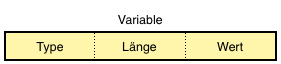
\includegraphics[scale=1]{Bilder/BasicEncodingRules}
	\caption{Darstellung eines Wertes in den Basic Encoding Rules}
\end{figure}

\subsection*{Der Type}
Der Datentype wird normalerweise mit einem Byte bestimmt. Doch von diesem Byte sind die 3 höchsten Bit reserviert. So kann es vorkommen, dass der Datentype mit mehreren Bytes beschrieben wird. Mit fünf Bits können nur 31 verschiedene Typen definiert werden.
\linebreak
\begin{figure}[h]
	\centering
	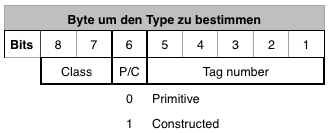
\includegraphics[scale=1]{Bilder/Datentype-BER}
	\caption{Die Verwendung der einzelnen Bits im Byte Datentype}
\end{figure}
\linebreak
Die Datentypen lassen sich in vier Klassen einteilen. Die Klassen sind Universal, Application, Context-specific und Private. Sie werden in den beiden höchsten Bits 7 und 8 dargestellt.
\linebreak
\begin{center}
	\begin{tabular}{| l | c | c |}
		\hline
		Klasse & Bit 8 & Bit 7\\
		\hline
		Universal & 0 & 0\\
		Application & 0 & 1\\
		Context-specific & 1 & 0\\
		Private & 1 & 1\\
		\hline
	\end{tabular}
\end{center}

\subsection*{Die Länge}
Die Länge des Datums kann in drei verschiedenen Varianten auftreten. Sie kann in kurzer oder in langer Form angegeben werden. Beide sind definit. Beide geben die Länge des Datums in Bytes an. Die dritte Form is indefinit. Es wird keine Länge angegeben. Das Ende des Datums wird markiert mit einer „end-of-contents“ Marke. Dazu werden zwei leere Bytes am Ende des Datums angehängt.
\linebreak
Die einfachste Form, mit der die Länge eines Datums bestimmt wird, ist definit und ein Byte lang. Dazu muss das höchste Bit im Byte 0 sein. In den restlichen 7 Bits kann die Länge des Datums in Bytes eingetragen werden. Dadurch, dass das höchste Bit 0 sein muss, liegt der Wertebereich nur bei 0 - 127 Bytes.
\begin{center}
	\begin{tabular}{| l | l |}
		\hline
		Bit 8 & Bit 7-1\\
		\hline
		0 & Die Anzahl an Bytes\\
		\hline
	\end{tabular}
\end{center}

\subsection*{Das Datum}
Das Datum selbst wird byteweise eingetragen, wobei mit dem höchsten Byte begonnen wird. Das niederste Byte komm zuletzt. Die Anzahl der Bytes muss mit der Längenangabe übereinstimmen.

% -------------
\pagebreak
% -----------------------------------------------------------------------------------------------------------------------------------------
% Literaturverzeichnis
% -----------------------------------------------------------------------------------------------------------------------------------------
\begin{thebibliography}{10}
	\bibitem{history}			% Geschichte
	\begin{small}
		www-i4.informatik.rwth-aachen.de/content/teaching/proseminars/sub/2003\_ss\_proseminar\_docs/snmp.pdf
	\end{small}
	\bibitem{netmanagement}	% Netzwerk Management
		Kurose, J. F.,
		Computernetze: Ein Top-Down-Ansatz mit Schwerpunkt Internet,
		Addison-Wesley,
		2002
	\bibitem{basicEncodingRules}	% Basic Encoding Rules BER
		www.rane.com/note161.html
\end{thebibliography}

\end{document}